\chapter{Scenarios de test et validation}

\section{Introduction du chapitre}
Ce chapitre formalise la strategie de verification adoptee pour demontrer le comportement securitaire de la solution. Il relie chaque test a une propriete Zero Trust attendue et identifie les preuves a collecter pour la validation.

\section{Strategie de test}
La validation repose sur des tests orientes preuve, executes de bout en bout sur les parcours critiques de securite.

Trois familles de tests sont retenues:
\begin{itemize}
	\item \textbf{Tests fonctionnels}: verification du cycle de vie des demandes (creation, approbation, expiration).
	\item \textbf{Tests de securite}: verification du refus par defaut et de l'acces temporaire strictement controle.
	\item \textbf{Tests de tracabilite}: verification de la presence des evenements dans les logs et tableaux de bord.
\end{itemize}

Chaque test est documente avec: preconditions, etapes, resultat attendu, resultat observe et preuves (captures/logs).

\section{Contexte d'execution des tests}
Tous les tests ont ete realises sur une machine virtuelle Azure hebergeant l'ensemble de la plateforme en conteneurs Docker. Les services sont segmentes en plusieurs reseaux Docker (proxy, IAM, cible SSH, Wazuh), avec un proxy inverse en frontal pour l'exposition controlee des interfaces web.

Ce contexte est important pour l'interpretation des resultats:
\begin{itemize}
	\item la connectivite reseau inter-service est gouvernee par les reseaux Docker et non par un flat network;
	\item la cible SSH est isolee dans son domaine de communication et n'est accessible qu'apres activation ACL;
	\item la collecte de logs vers Wazuh est verifiee dans le meme environnement de production maquette.
\end{itemize}

\section{Cas de test IAM/PIM/PAM}
\subsection{TC-01: Authentification forte IAM}
\textbf{Preconditions}: utilisateur actif dans Authentik et MFA configure.

\textbf{Etapes}:
\begin{enumerate}
	\item ouvrir la page de connexion de l'application;
	\item saisir identifiant et mot de passe;
	\item valider le second facteur TOTP.
\end{enumerate}

\textbf{Attendu}: acces accorde uniquement apres validation MFA.

\textbf{Preuves}: capture login, capture ecran MFA, event d'authentification.

\begin{figure}[H]
	\centering
	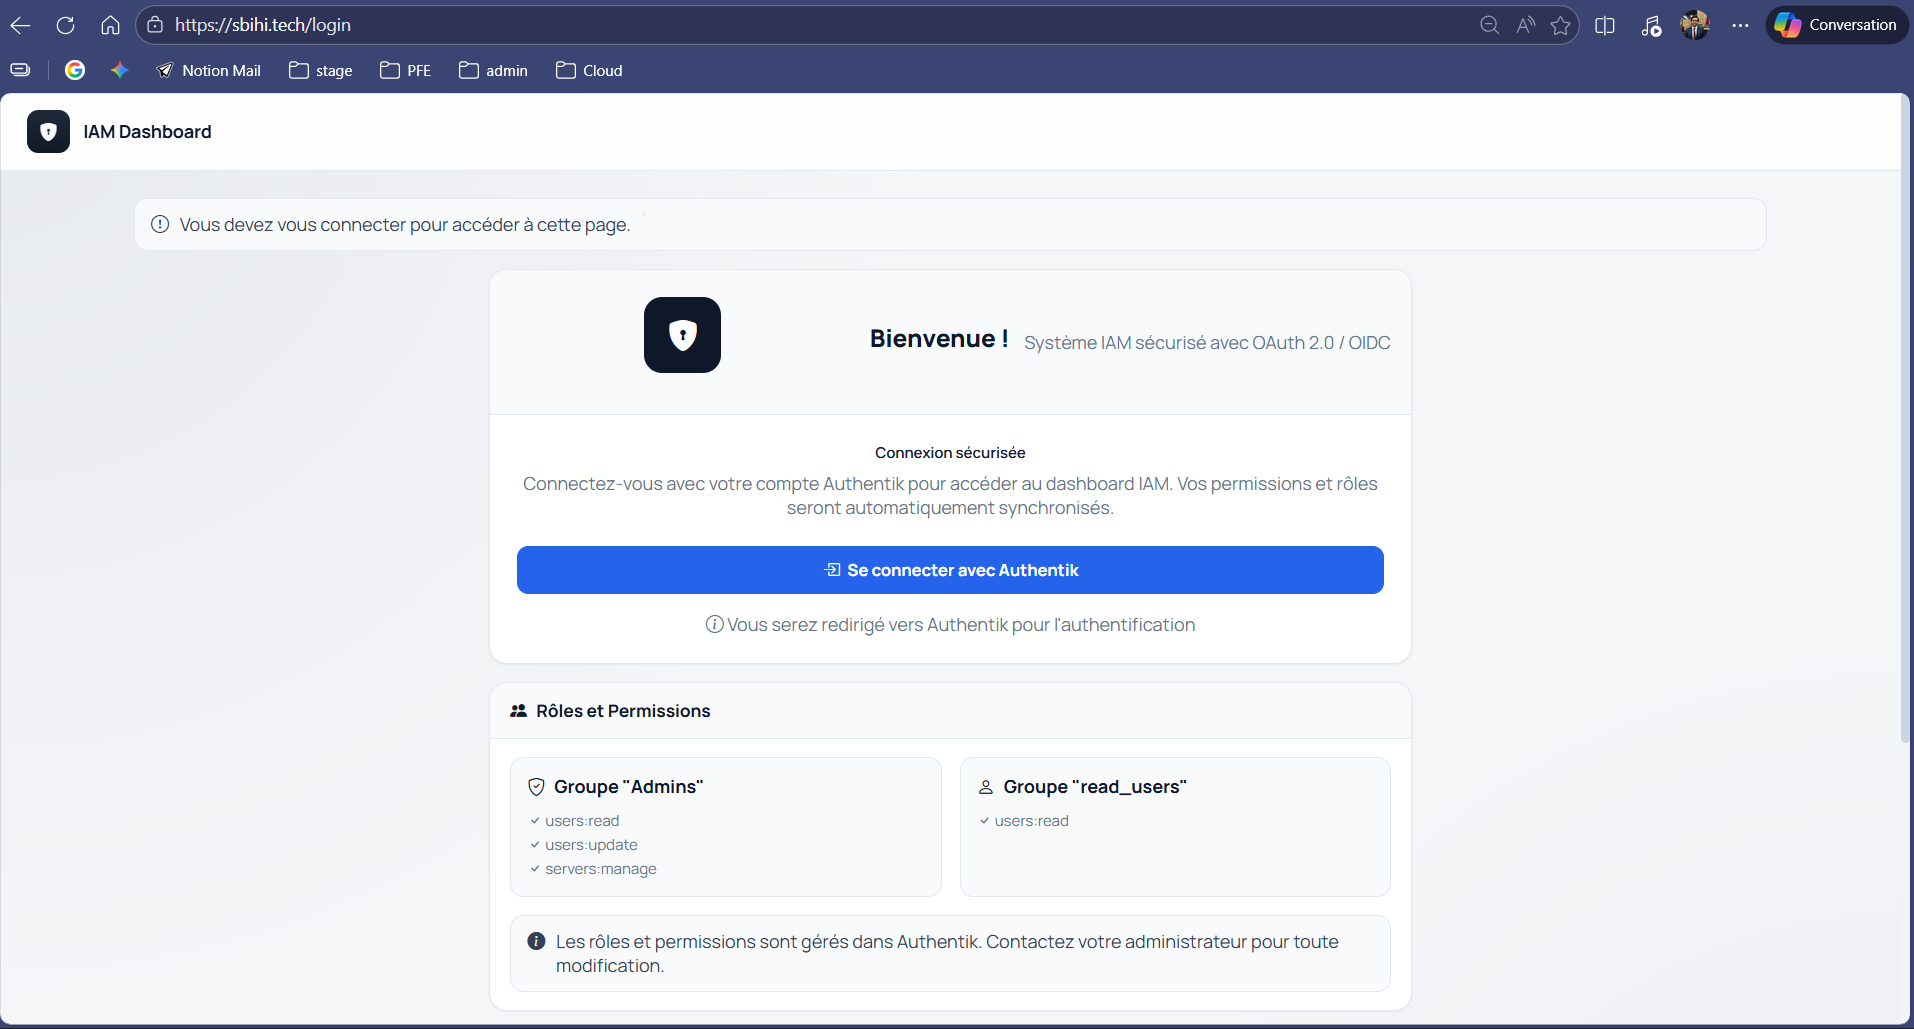
\includegraphics[width=0.9\textwidth]{images/iam_dashbord_login.png}
	\caption{Preuve TC-01: ecran de connexion IAM avant emission d'une session valide.}
	\label{fig:tc01-login}
\end{figure}
Cette image confirme que le point d'entree du systeme passe par la couche IAM. Dans la logique Zero Trust, cette etape est indispensable pour associer toute action ulterieure a une identite authentifiee.

\subsection{TC-02: Creation d'une demande JIT}
\textbf{Preconditions}: utilisateur sans acces privilegie permanent sur la cible.

\textbf{Etapes}:
\begin{enumerate}
	\item se connecter a l'interface utilisateur;
	\item soumettre une demande d'acces a une machine cible;
	\item tenter de soumettre une deuxieme demande identique si la premiere est \texttt{pending}.
\end{enumerate}

\textbf{Attendu}: la premiere demande passe \texttt{pending}; la seconde est bloquee par regle anti-doublon.

\textbf{Preuves}: capture dashboard user, capture message de blocage anti-doublon.

La validation de ce cas repose sur l'existence d'un controle anti-doublon cote application. Ce controle evite les demandes paralleles contradictoires et stabilise la gouvernance des droits temporaires.

\subsection{TC-03: Approbation admin et activation ACL}
\textbf{Preconditions}: demande \texttt{pending} visible cote administration.

\textbf{Etapes}:
\begin{enumerate}
	\item ouvrir le dashboard admin;
	\item approuver la demande;
	\item verifier le statut et la date d'expiration;
	\item verifier la mise a jour de la politique ACL.
\end{enumerate}

\textbf{Attendu}: statut \texttt{approved}, ACL active, fenetre TTL demarree.

\textbf{Preuves}: capture action admin, capture ACL apres approbation, trace applicative.

\begin{figure}[H]
	\centering
	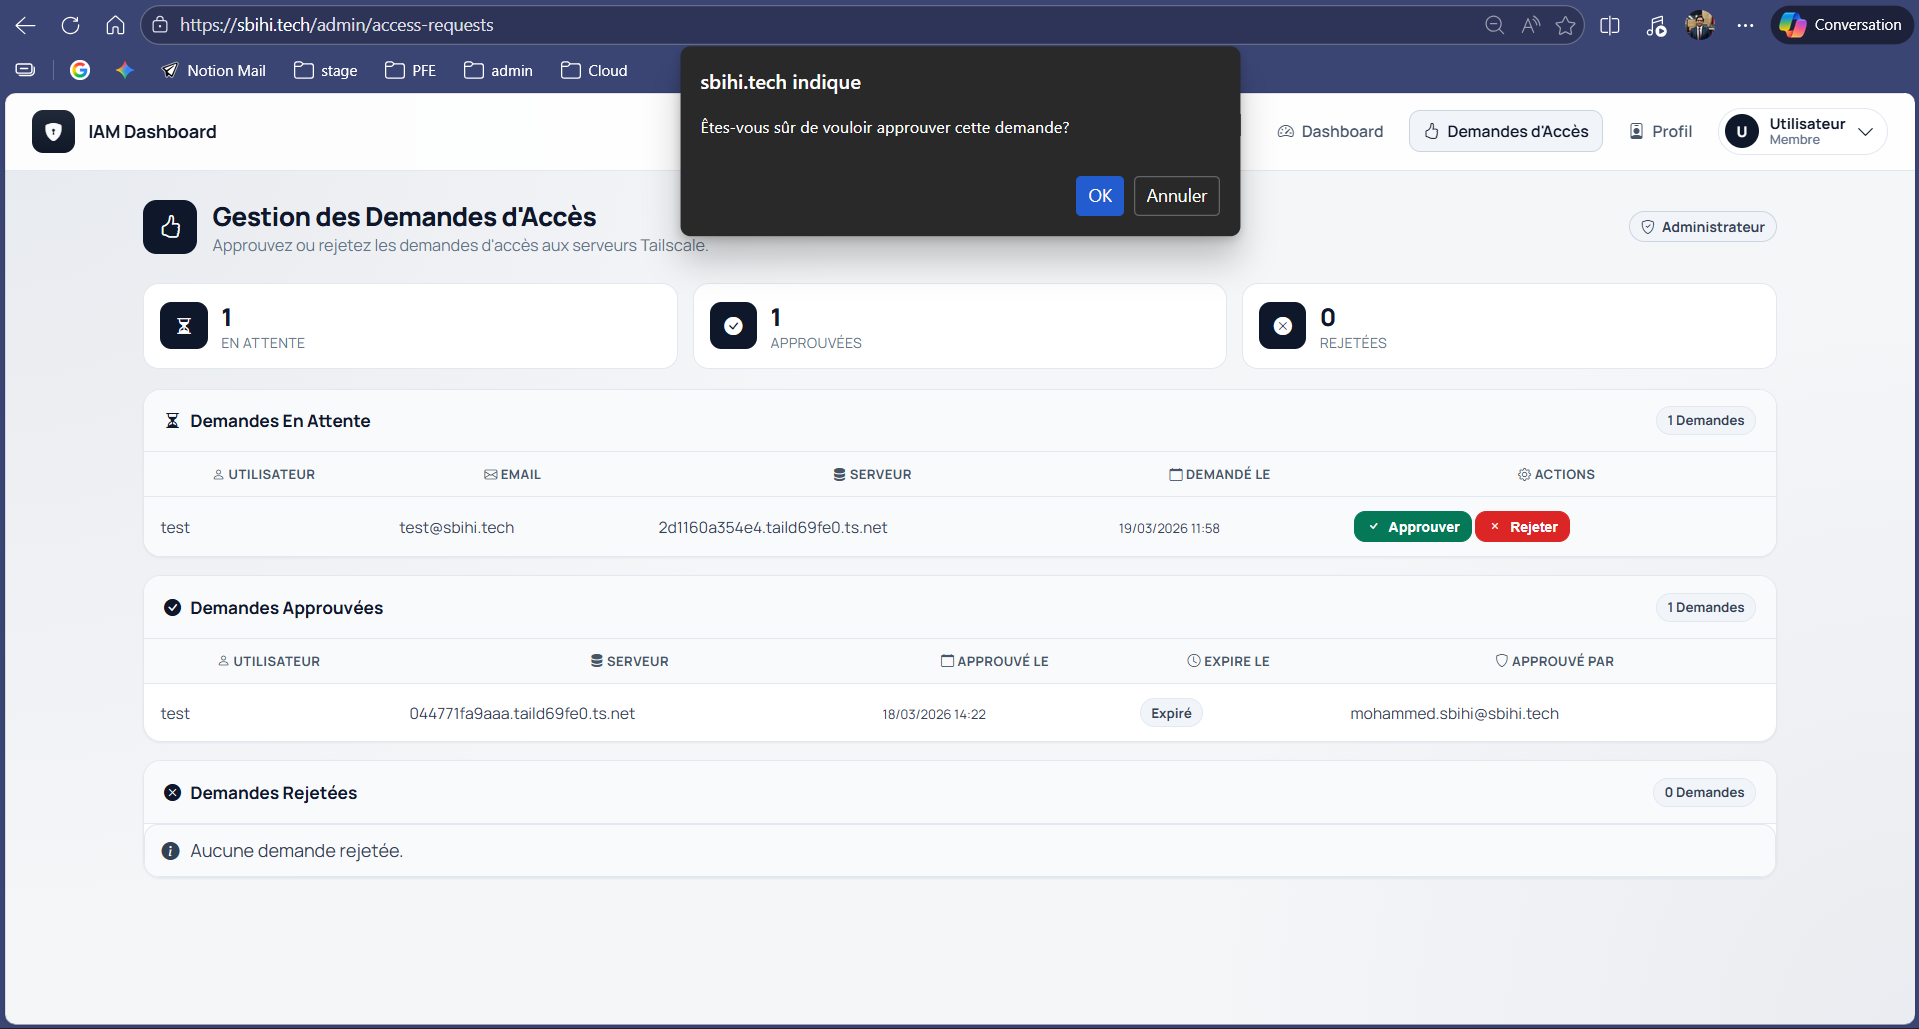
\includegraphics[width=0.95\textwidth]{images/approuve_request_by_admin.png}
	\caption{Preuve TC-03: action d'approbation executee par l'administrateur.}
	\label{fig:tc03-admin-approval}
\end{figure}
La capture montre que l'activation du droit est le resultat d'une decision humaine explicite. Cette etape introduit une validation de gouvernance avant toute modification reseau effective.

\begin{figure}[H]
	\centering
	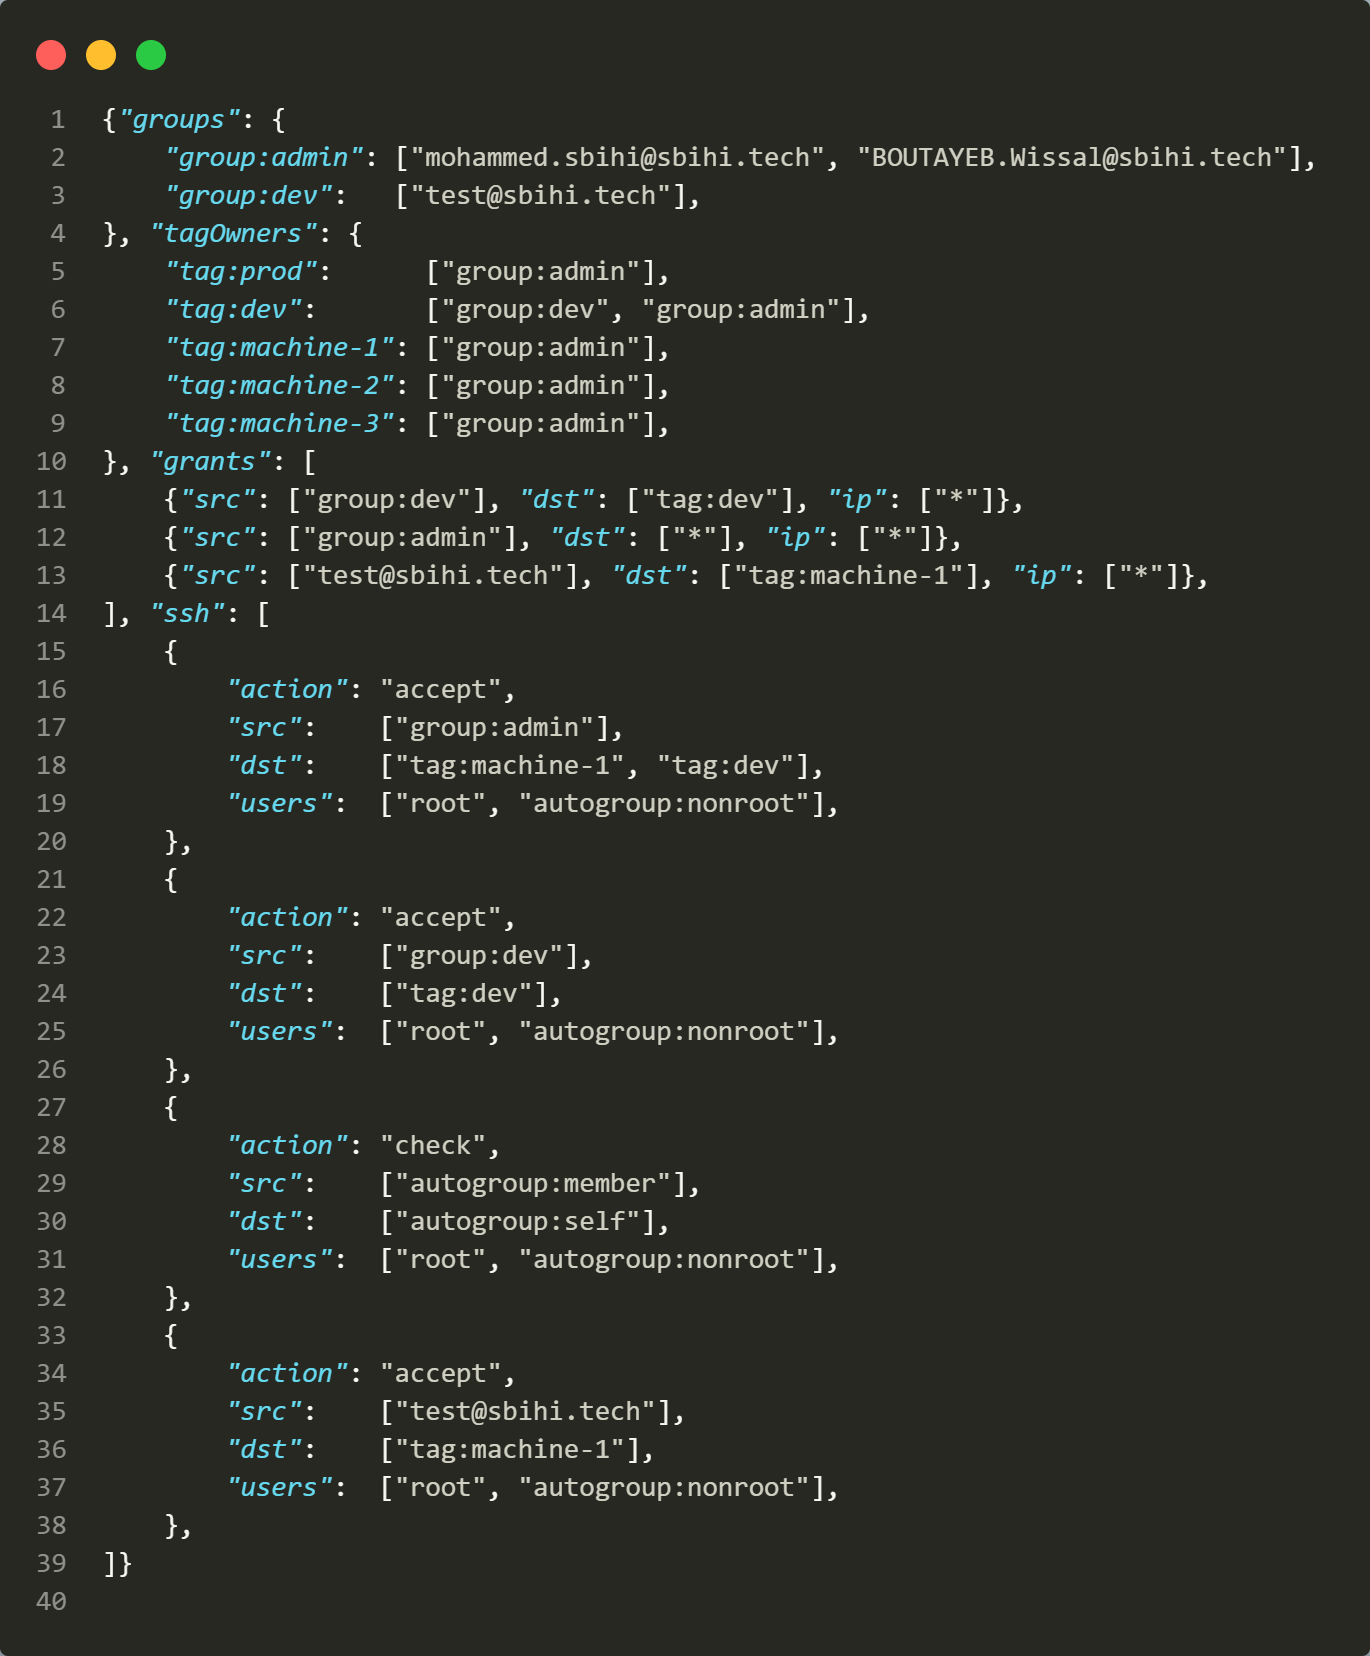
\includegraphics[width=0.95\textwidth]{images/acl-after-acces-granted.png}
	\caption{Preuve TC-03: regle ACL active apres approbation de la demande.}
	\label{fig:tc03-acl-after}
\end{figure}
L'evolution de la politique ACL apres approbation demontre le chainage correct entre workflow applicatif et enforcement reseau. Cette coherence est centrale pour prouver l'efficacite du mecanisme JIT.

\subsection{TC-04: SSH avant et apres approbation}
\textbf{Preconditions}: une cible SSH integree et une demande en cours de traitement.

\textbf{Etapes}:
\begin{enumerate}
	\item tenter une connexion SSH avant approbation;
	\item approuver la demande;
	\item retenter la connexion SSH pendant la fenetre active.
\end{enumerate}

\textbf{Attendu}: echec avant approbation, succes apres approbation.

\textbf{Preuves}: captures terminal avant/apres, logs de connexion.

\begin{figure}[H]
	\centering
	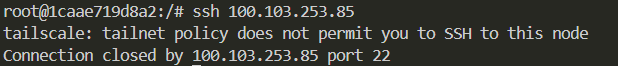
\includegraphics[width=0.98\textwidth]{images/ssh_failed_before_from user test@sbihi.tech to a other machine in the tailscale network.png}
	\caption{Preuve TC-04 (avant approbation): tentative SSH refusee car aucun droit temporaire n'est encore actif.}
	\label{fig:tc04-ssh-failed-before}
\end{figure}
Le refus observe avant approbation valide le comportement attendu en mode \textit{deny by default}. L'infrastructure applique bien l'absence de confiance implicite envers les utilisateurs non autorises.

\begin{figure}[H]
	\centering
	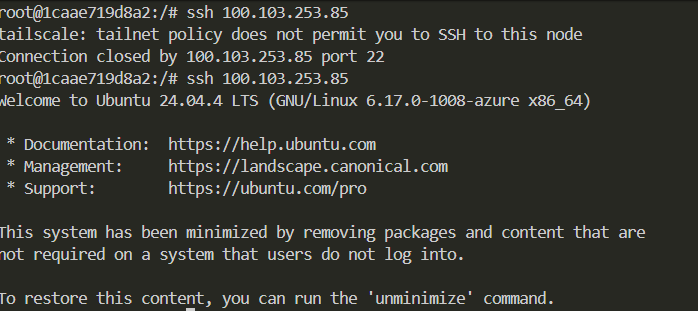
\includegraphics[width=0.98\textwidth]{images/ssh_accepted_before_from user test@sbihi.tech to a other machine in the tailscale network.png}
	\caption{Preuve TC-04 (apres approbation): tentative SSH acceptee pendant la fenetre d'acces JIT.}
	\label{fig:tc04-ssh-success-after}
\end{figure}
Le succes de connexion apres approbation confirme la levée de restriction strictement conditionnee. Ce comportement binaire avant/apres est la preuve la plus lisible de l'efficacite du couple approbation admin + ACL dynamique.

\subsection{TC-05: Expiration automatique et revocation}
\textbf{Preconditions}: acces \texttt{approved} avec TTL court.

\textbf{Etapes}:
\begin{enumerate}
	\item attendre l'expiration ou lancer le script de nettoyage;
	\item verifier le passage au statut \texttt{expired};
	\item retenter une connexion SSH.
\end{enumerate}

\textbf{Attendu}: acces revoque, ACL retiree, connexion SSH refusee.

\textbf{Preuves}: sortie script \texttt{cleanup}, capture SSH refuse, log d'expiration.

Ce cas final est critique, car il valide la non-persistance des privileges. L'absence de nettoyage automatique annulerait le benefice Zero Trust et recreerait un risque d'acces permanent.

\subsection{TC-06: Tracabilite Wazuh des commandes SSH}
\textbf{Preconditions}: connexion SSH active sur la machine cible et agent Wazuh operationnel.

\textbf{Etapes}:
\begin{enumerate}
\item executer des commandes shell sur la cible pendant une fenetre JIT autorisee;
\item verifier l'ecriture des traces dans \texttt{/var/log/auth.log};
\item confirmer la remontee des evenements dans le dashboard Wazuh.
\end{enumerate}

\textbf{Attendu}: les commandes executees apparaissent dans Wazuh avec le contexte utilisateur/source.

\textbf{Preuves}: capture Wazuh de logs SSH centralises.

\begin{figure}[H]
	\centering
	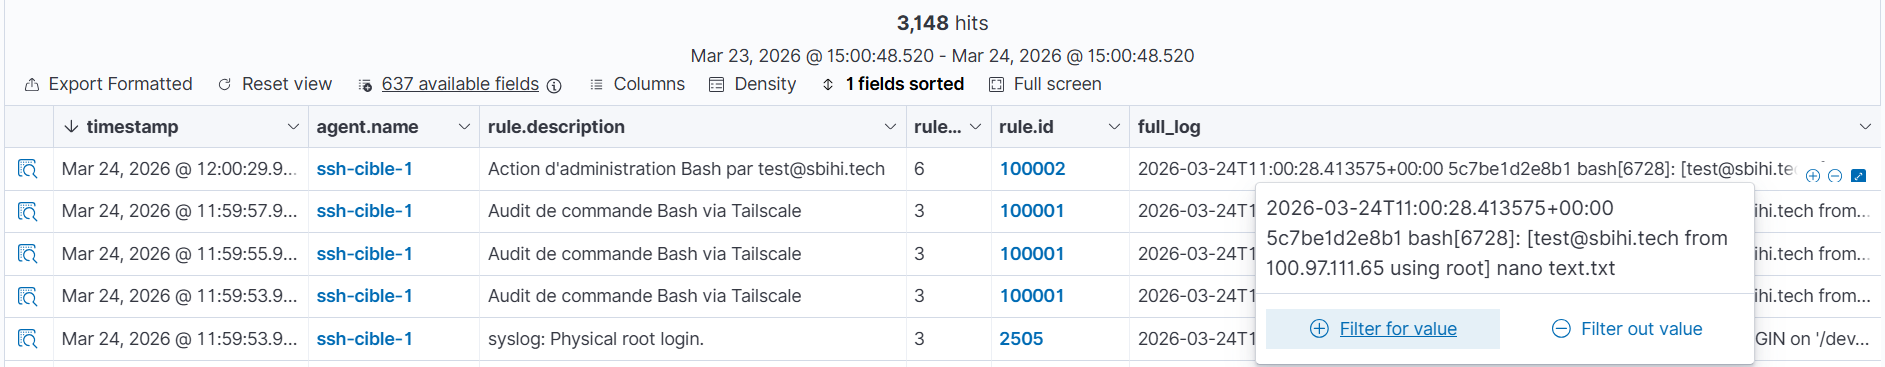
\includegraphics[width=0.97\textwidth]{images/wazuh_log_from ssh showing what the user did in after login to the ssh cible .png}
	\caption{Preuve TC-06: evenements Wazuh issus des commandes SSH journalisees sur la machine cible.}
	\label{fig:tc06-wazuh-ssh-audit}
\end{figure}
Ce test valide la chaine de tracabilite de bout en bout: commande utilisateur -> journal cible -> ingestion agent -> visualisation SIEM Wazuh.

\section{Resultats de validation}
Les tests attendus doivent confirmer les proprietes suivantes:
\begin{itemize}
	\item aucune elevation de privilege sans authentification forte;
	\item aucune activation de droit sans approbation explicite;
	\item aucune persistance d'acces au-dela de la fenetre autorisee;
	\item auditabilite de l'ensemble du cycle demande-approbation-expiration, incluant les commandes shell sur machine cible.
\end{itemize}

La section sera finalisee avec les resultats observes, les captures associees et les eventuelles non-conformites detectees durant les essais.

Les preuves inserees confirment la logique attendue par le modele Zero Trust: refus par defaut, autorisation explicite et temporalite stricte des privileges.

\section{Conclusion du chapitre}
La campagne de test proposee couvre les points critiques du cycle JIT: refus par defaut, approbation explicite, acces temporaire et revocation automatique. Ces verifications constituent la base de mesure des resultats presentes au chapitre suivant.
